\chapter{Satellite Constellation Management Tools} \label{chapter_tools}
This chapter presents all the tools developed along this work to achieve the purposes of the thesis.



\section{Orbit Propagators} \label{orbit_propagators_par}
Applications and topics covered by this thesis clearly require an orbital propagator to be studied.
All the propagators produced along this work exploit the Cowell's model shown in subsection \ref{orbit_prop_paragraph}.
Both undisturbed and perturbed motion have been analysed.

Orbit propagators must take in input the following data:
\begin{itemize}
    \item \textbf{Initial orbit}. The initial state of the staellite orbit must be defined before propagation.
          All the six orbital elements (see subsection \ref{sat_state_rep_paragraph}) and the epoch are required. 
          The scripts can also work defining the six components of position and velocity vectors.
          Even the TLE can be set as input, which will be appropriately converted into the classical elements representation.  
    \item \textbf{Spacecraft specifications}. According to the features of the selected propagator, one or more satellite characteristics shall be provided when considering perturbations.
          For instance, in presence of atmospheric drag, $C_D$ and $BC$ (which means cross-sectional area and mass) are needed. 
          The reflectivity coefficient must be added if the problem takes into account the SRP.
    \item \textbf{Time settings}. These input parameters include \textit{time frame} and \textit{time step}.
          The first one simply consists of the total temporal period of propagation requested by the user.
          On the other hand, the time step is strictly related to the output accuracy.
          Lower values imply more accurate results, as well as longer computation times.
          In a nutshell, the outputs will be discretized in as many points as those deriving from the ratio between time frame and time step.
          The accuracy of the model is actually always the same. 
          The difference lies in the shape of the outputs: small time steps provide narrower plots. 
          Figure \ref{time_step_fig} shows the SMA of a LEO satellite propagated for one orbit that lasts approximately 50 minutes. The assigned time step is of 5 minutes (the curve is therefore discretized into 10 points).
    \item \textbf{Perturbations parameters}. Propagators that involve any perturbing acceleration need the parameters which describe that force. 
          For example, the perturbing specific force of atmospheric drag (equation \ref{eq:drag_acc}) requires the air density, which will be given by a specific atmospheric model.
          Even for the acceleration of an eventual thruster it is necessary to specify the force it generates.
\end{itemize}

\begin{figure}[h]
      \centering
      %\textbf{Your title}\par\medskip
      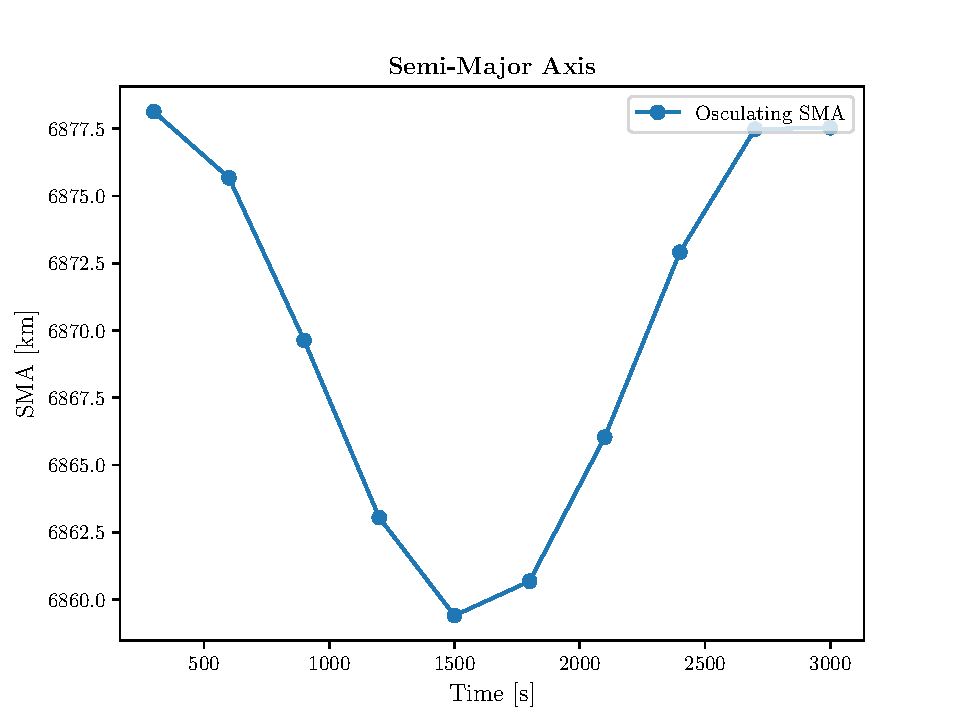
\includegraphics[scale=0.8]{img/time_step.pdf}
      \caption{Osculating SMA of a LEO satellite during one orbit. Propagation time settings: time step = 5 minutes, time frame = 50 minutes.}
      \label{time_step_fig}
  \end{figure}


\subsection{Undisturbed Motion}
The first orbit propagator proposed by this thesis consists of the ideal motion of a spacecraft neglecting all the possible perturbations that might affect it.
Therefore, this kind of propagation is governed by the two-body equation shown in subsection \ref{twobody_par}.

This model is mainly useful for two reasons.
First, it requires computation times definitely shorter than a perturbed propagation, allowing quick results when perturbations are not considered decisive for the purposes of the user.
Secondly, it provides an educational method to better understand the perturbing effects when compared to more realistic propagators.

Figure \ref{kep_low_ecc_fig} shows the orbital elements values of the motion of a satellite in LEO.
\begin{figure}[h]
      \centering
      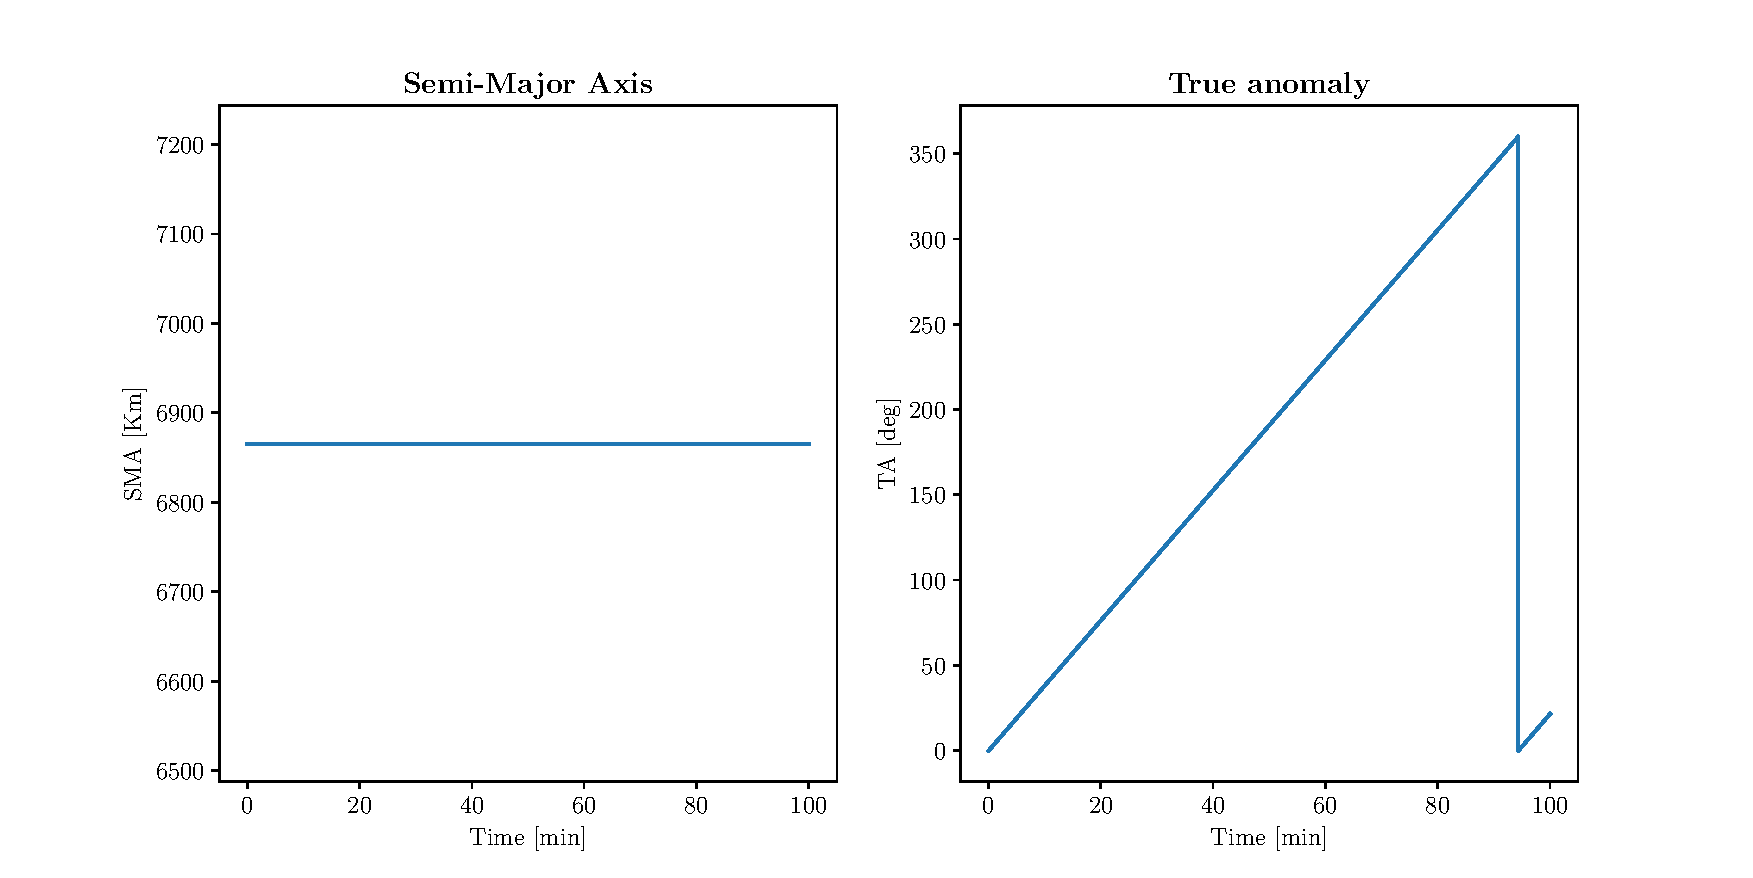
\includegraphics[scale=0.5]{img/keplerian_elements_low_ecc.pdf}
      \caption{SMA and true anomaly variation along around one LEO satellite orbit with eccentricity of 0.001}
      \label{kep_low_ecc_fig}
\end{figure}
Only SMA and true anomaly are reported for matters of layout.
The graph of the other elements is constant like the semi-major axis, because no perturbation affects their behavior.
The true anomaly is the only time-variant parameter, and in this case its curve looks like varying constantly.
The reason of this aspect lies in the eccentricity: this example is characterized by a near-circular orbit, therefore the velocity of the satellite is almost the same along the entire orbit.
Increasing the eccentricity value, like in figure \ref{kep_high_ecc_fig}, the true anomaly changes more rapidly when is in proximity of the perigee and vice-versa.
\begin{figure}[h]
      \centering
      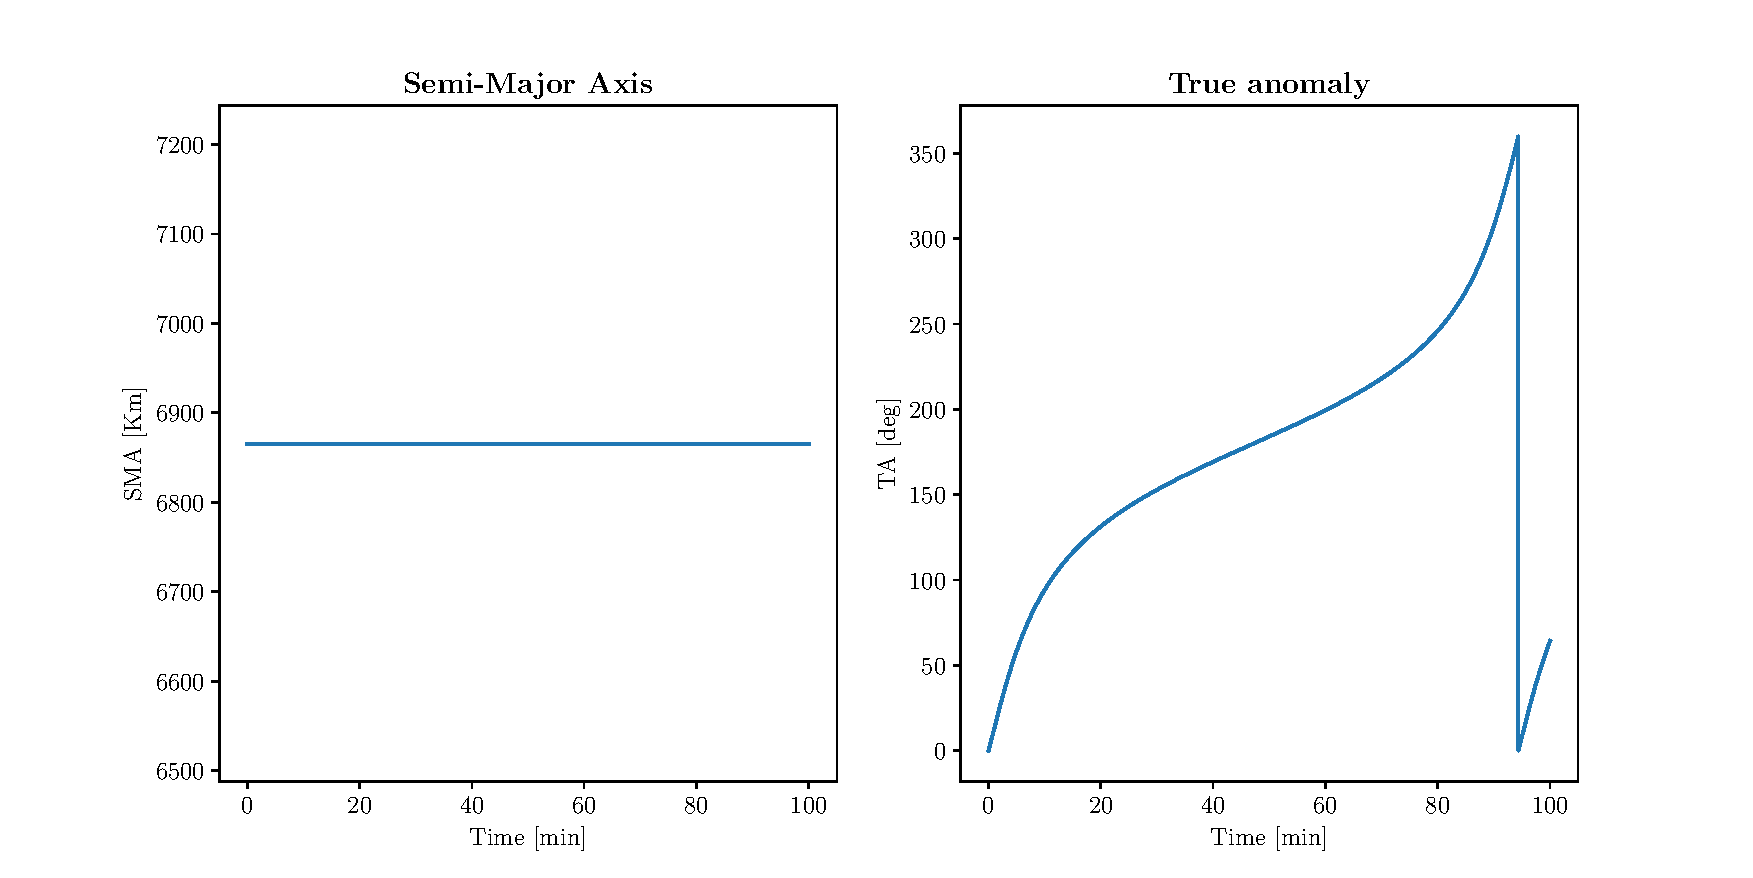
\includegraphics[scale=0.5]{img/keplerian_elements_high_ecc.pdf}
      \caption{SMA and true anomaly variation along around one LEO satellite orbit with eccentricity of 0.5}
      \label{kep_high_ecc_fig}
\end{figure}

All the case studies of this research consist of near-circular orbits.
Despite the fact that zero-eccentricity condition is not feasible, this comparison demonstrates that very low values of eccentricity make the assumption of circular orbit highly acceptable.  


\subsection{Perturbations}
The propagators developed by this work which take into account perturbing effects are based on the Cowell's technique of subsection \ref{orbit_prop_paragraph}.

Since Sun-synchronous orbits at low altitudes denote the main discussion point of this thesis, Earth's oblateness and atmospheric drag represent the perturbations of greatest interest. 
However, propagations with SRP and 3rd-body forces have been examined as well for assessing long-term effects. 

The perturbing acceleration functions performed by this thesis come from poliastro's library.

\subsection{Atmospheric Models}
Atmospheric drag exponential model has been found to be too approximate compared to the results provided by GMAT of same examples.
For that reason, two more accurate atmospheric models have been implemented into the scripts designed along this work.
The first one consists of COESA76 model, while the second is the JB2008 one.
Their theoretical background has been already exposed in paragraph \ref{orbit_prop_paragraph}.
JB2008 is definitely the most accurate model


\subsection{Mean Orbital Elements Converter}
\subsection{Sun Synchronous Orbits Functions}
\subsection{Satellite Constellation Propagator}

\section{Revisit Time Collector}
The revisit time collector (RTC) tool intends to compute the amount of passages of a satellite above a specific position on Earth.
It collects the \textit{access times} of the spacecraft when its target on the ground is within the area delimited by the swath width of the satellite's on-board camera. 
It can work with a single space vehicle or with a constellation. 
In the latter case, the script provides all the access times taking into account every single satellite of the pattern. 

In addition to the input parameters required by the selected propagator (paragraph \ref{orbit_propagators_par}), the RTC needs the target coordinates in latitude and longitude, as well as the swath width of the electro-optical sensor.
The algorithm computes the distance between the sub-satellite point on the ground and the target at each time step.
This calculation is performed considering some meaningful aspects.

The goal of the RTC clearly requires the estimation of the satellite's position in an ECEF reference frame.
If its motion was evaluated with respect to an ECI system, the ground track of the orbit would be always the same after each orbital period.
ECEF coordinates shall be then converted into the geodetic latitude-longitude location of the spacecraft's subpoint in order to proceed with the distance calculation.

The computation of the distance between two points on the Earth surface shall take into account the sphericity of the planet.
To accomplish this condition, the algorithm computes the so-called geodesic distance, which can be defined as the shortest path between two points on the surface of an ellipsoidal model of the Earth. 
As regards the geodetics, the script takes advantage of the method proposed by Karney \cite{karney2013algorithms}.

Summarizing, the algorithm extracts the sub-point latitude and longitude from the ECEF state vector of the satellite and, after that, calculates the geodesic distance with respect to the ground target.
This path is then compared with half the value of the potential swath width (PSW) at each time step of the propagation.
If the distance is smaller than PSW then the script saves the epoch related to that time step.

\begin{algorithm}
      \caption{\textbf{Revisit Time Collector algorithm}}
      \begin{algorithmic}[1]
            \Procedure{Collect revisit time epochs over a specific target}{} 
                  \State propagate the satellite's orbit for the desired time frame
                  \For{each time step in the time frame}
                        \State convert satellite state vector from ECI to ECEF
                        \State extract geodetic latitude and longitude
                        \State compute the geodesic distance between target and sub-satellite point
                        \If{distance between the two points < $\frac{PSW}{2}$}
                              \State collect the epoch of the current time step
                        \EndIf
                  \EndFor
            \EndProcedure
      \end{algorithmic}
\end{algorithm}

It is important to underline that the actual sensor input value to be implemented in the RTC should be related to the concept of \textit{potential swath coverage}.
It identifies the potential path reachable by a pointable space system.
If the satellite can not work off-nadir then the input parameter will be simply equal to half the SW due to the fact that the subpoint always lies in the middle of the observed area.
Therefore, according to the figure \ref{potential_sw_fig}, a proper use of the algorithm should get half the potential swath width (PSW) as input value.
\begin{figure}[H]
      \centering
      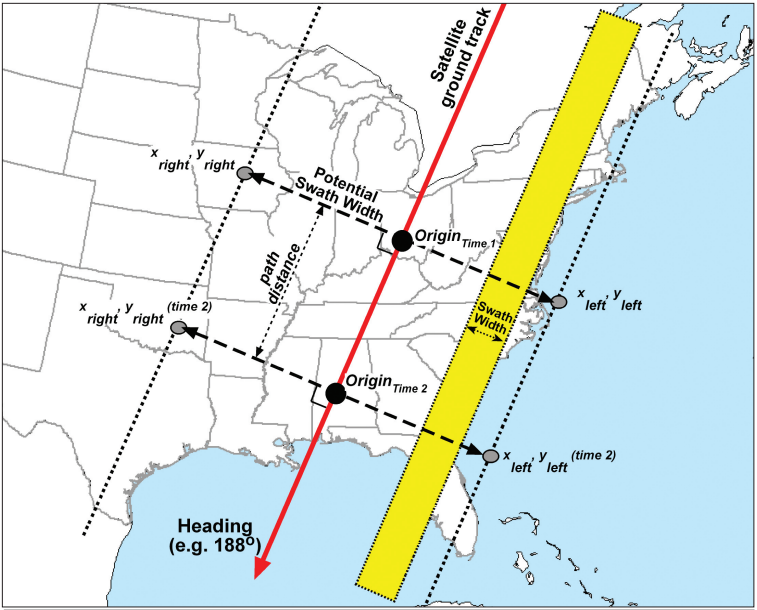
\includegraphics[scale=0.6]{img/potential_sw.png}
      \caption{Projection of satellite ground track and potential swath width with respect to its swath width at two time steps \cite{hodgson2008modeling}.}
      \label{potential_sw_fig}
\end{figure}


\section{Station-Keeping Simulator}
This station-keeping simulator aims to perform the altitude and inclination maintenance of low-thrust propelled satellites.
The tool combines the orbit propagator and an algorithm that keep the spacecraft within a defined range of altitudes and inclinations.
The required input parameters include the thrust force of the propulsion system as well as the edge values of the orbital elements that define the station-keeping box.
The simulator works with the perturbations, therefore it is indispensable to deal with the mean orbital elements to carry out the maintenance.
The logic behind the method is shown below.
\begin{algorithm}[H]
      \caption{\textbf{Station-Keeping Simulator}}
      \begin{algorithmic}[1]
            \Procedure{Simulate the absolute station-keeping of a spacecraft}{} 
                  \For{each time step in the time frame}
                        \State propagate the satellite's orbit
                        \If{current mean SMA < lower SMA}
                            \While{current mean SMA < upper SMA}
                                \State activate thruster
                            \EndWhile
                        \EndIf           
                        \If{current mean inclination < lower inclination}
                            \While{current mean inclination < upper inclination}
                                \State activate thruster
                            \EndWhile
                    \EndIf
                  \EndFor
            \EndProcedure
      \end{algorithmic}
\end{algorithm}
The algorithm uses the Edelbaum-Kechichian theory reported in subsection \ref{station_keeping_par}.
However, a careful observer would notice that actually the script takes advantage of this theory only to compute the yaw angle (equation \ref{yaw_angle_equation}) in case of out-of-plane maneuver (change in inclination).
Indeed, the burning time estimated by the equations is never taken into account.
The update of the satellite's position at each time step allows a better accuracy which otherwise would be affected by the uncertainties generated by the unpredictable factors of the perturbing effects over a long time frame.

Nevertheless, the equations of the Kechichian's method are used to provide the $\Delta V$ required by the station-keeping, which is a fundamental parameter for the mission designer.


\section{Differential Drag Controller}
The differential drag algorithm represents the main effort of this thesis.
It consists of a method to perform the phasing through the differential drag of two or more satellites, of any shape and mass, after their deployment at the beginning of the mission.
The goal is to achieve an assigned orbital slot and same mean semi-major axis respectively on all spacecraft forming the constellation, resulting in zero relative velocity between them.

\subsection{Planet's Control Algorithm}
Since the algorithm designed by this thesis takes inspiration from the controller adopted by Planet, a description of the latter is presented.
The objective of Planet's algorithm is the same as that of the thesis.
It consists of labeling the satellite in the lowest orbit as the leading satellite.
Then, a two-component state composed by the mean Earth-centered angular distance to its desired slot $\theta_i$, and the angular velocity $\dot{\theta}_i$ relative to the leader, is computed for each trailing satellite.
The procedure is reported below in the identical form presented by the company \cite{foster2015orbit}.

\begin{algorithm}[H]
      \caption{\textbf{Planet's Control Algorithm}}
      \begin{algorithmic}[1]
            \Procedure{Create high-drag windows}{} 
                  \State remove any previously issued high-drag windows
                  \State compute $\theta_i$, $\dot{\theta}_i$ of each satellite \textit{i} relative to previous leader (mean, not osculating)
                  \State compute $\ddot{\theta}$ of a satellite in high-drag vs. low-drag mode
                  \State assign leader to be satellite with greatest $\dot{\theta}$ (i.e. lowest altitude)
                  \For{each satellite \textit{i} that is not the leader}
                        \State offset $\theta_i$, $\dot{\theta}_i$ to be relative to new leader: $\theta_i = \theta_i - \theta_{leader}, \dot{\theta}_i = \dot{\theta}_i - \dot{\theta}_{leader}$
                        \State get required high-drag duration to null relative speed with leader: $\Delta t_{i,hd} = - \frac{\dot{\theta}_i}{\ddot{\theta}}$
                        \State get angle travelled during desired high-drag window: $\theta_{i,hd} = \frac{1}{2} \ddot{\theta} \Delta t_{i,hd}^2$
                        \State get wait time to target desired slot: $\Delta t_{i,wait} = \frac{\theta_{i,hd} - \theta_i}{\dot{\theta}_i}$
                        \State create high-drag window for satellite \textit{i} starting at $t_{now} + \Delta t_{i,wait}$ for duration $\Delta t_{i,hd}$
                  \EndFor
            \EndProcedure
      \end{algorithmic}
\end{algorithm}

The strategy is to first obtain the high-drag time $\Delta t_{i,hd}$ (high-drag window) needed by the trailing satellite for matching the leader's semi-major axis.
Next, the amount of time $\Delta t_{i.wait}$ each spacecraft has to wait in the low-drag configuration before the high-drag window is initiated is computed.
\cite{foster2015orbit}













It is absolutely necessary the use of the mean orbital elements over all the phases of the script.
This tool assumes that the space vehicles involved have the same initial orbital elements except SMA and argument of latitude.  
In the following explanation of the algorithm two identical spacecraft will be considered.

First of all, the algorithm needs to establish a reference vehicle, the \textit{leading satellite}, which will be identified by the spacecraft travelling in the lowest orbit (lower mean SMA).
On the other side, the \textit{trailing satellite} is the one with the highest altitude.
In addition to the initial in-orbit positions, the tool requires the BC related to the various drag profiles the satellite can achieve.
Moreover, the user shall indicate the desired relative angular path between the spacecraft.
For simplicity, only two attitude modes will be treated: high drag and low drag.
Figure \ref{low_vs_high_dragmode_fig} in chapter \ref{background_chapter} basically represents the problem at hand.
At this point, the algorithm's core begins.
The first calculation consists of the current angular distance from the trailing satellite to the desired placement with respect to the leader at the initial time step.
After that, two predictions are made.
First, the estimation of the necessary time for the trailing satellite in high drag to reach the same mean SMA of the leader.
The latter is set to nominal low drag during the entire operation.
Secondly, the strategy aims at evaluating the waiting time before performing the high drag attitude, in order to match the leader's altitude and the assigned phasing at the same time.

\begin{algorithm}[h]
      \caption{\textbf{Differential Drag Phasing}}
      \begin{algorithmic}[1]
            \Procedure{Perform phasing through differential drag}{} 
                  \State establish the leading satellite (smallest SMA)
                  \For{each trailing satellite of the constellation}
                        \For{each assigned iteration}
                              \State compute difference in mean anomaly with respect to the leader $\Delta n$
                              \State compute angle to reach the desired slot relative to the leader $\theta_{err}$
                              \State Assign and estimation time $t_{est}$ from $\theta_{err}$
                              \State estimate $\ddot{\theta}$ from high drag vs. low drag mode over $t_{est}$
                              \State estimate high drag time window $t_{hd} = \frac{\Delta n}{\ddot{\theta}}$
                              \State compute angle travelled during high drag window $\theta_{hd} = \frac{1}{2}\ddot{\theta}t_{hd}^2$
                              \State estimate waiting time window $t_{wait} = \frac{\theta_{err} - \theta_{hd}}{\Delta n}$
                              \State get new estimation time $t_{est} = f(t_{wait}, t_{hd}, h_{lead}, h_{trail})$ 
                        \EndFor
                        \For{each time step in $t_{wait}$}
                              \State propagate the leader in low drag mode
                              \State propagate the trailer in low drag mode
                        \EndFor
                        \For{each time step in $t_{hd}$}
                              \State propagate the leader in low drag mode
                              \State propagate the trailer in high drag mode
                        \EndFor
                  \EndFor
            \EndProcedure
      \end{algorithmic}
\end{algorithm}


